%!TEX root = ../main.tex

\chapter{Finding unreachable code using a SMT-Solver \textasciitilde 10 sites}
\label{cha:finding unreachable code using a smt-solver}
\emph{10 Sites}

The developed approach uses the \emph{Control-flow graph} as a basis like described in \ref{sec:building cfg}, but does not transform it into \emph{Single static Assignment} form.
During analysis the \emph{Control-flow graph} will be traversed and interpreted like the program will be executed.
After each interpretation state (e.g. \emph{Assignments}, \emph{Path Conditions}) will be added accordingly and must be taken into account.
Merging of state has to be handled correctly to make correct statements about the current value of a variable.
The state is represented in the form of a predicate, which may be checked by a system capable of determining satisfiability (e.g. an \emph{SMT-Solver}).
Satisfiable results will continue with the next block(s) and using the new state as a basis and flag this block as visitable.
Unsatisfiable results stop the computation at the current block and will not pursue to continue the path.
Therefore this method is pessimistic.
By using this method every error should be found in theory (as described in \ref{cha:conclusion}), since every instruction will be handled like during execution. 
This entails barriers such as: 
\begin{itemize}
	\item Significant increase in time needed for analysis. 
	\item Possibly exponentially growing expressions to determine satisfiability.
\end{itemize}
These problems lead to greater execution time, which requires the implementation of reactions (e.g. early stopping, assuming values for variables in loops).


\section{Translation of Functions}
\label{sec:translation}
For every function the \emph{Control-flow Graph} will be calculated and used as basis. Information about parameters and global-/system variables also need to be provided in order to handle Function-/Procedure-calls. 
Two separate procedures will be performed on this Control-flow Graph.
\begin{enumerate}
	\item \emph{Unreachable Code due to unconditional jumps} is relatively easy to find after the Control-flow Graph was created. Every Block (except the \emph{Begin Block}) which does not have any incoming edges must be unreachable.
		Note that these types of errors may also be found as described in section \ref{sec:analysis}, but were filtered out before.
	\item \emph{Unreachable Code due to infeasible conditions} needs a sophisticated and more expensive (in terms of computing resources) approach to identify. The following section \ref{sec:analysis} describes how to detect them.
\end{enumerate}
\subsection{Translation of Instructions}
% Types of instructions
Instructions come in three different types and must be marked accordingly:
\begin{enumerate}
	\item \emph{Assignments} are usually the most common form of instruction. They denote a change of the underlying value of a variable and therefore reset the state (of said variable) during analysis. 
	\item \emph{Conditions} occur only as the last instruction of a block from a \emph{Control-flow Graph}. Note that the last Instruction does not necessarily to be a \emph{condition}.
	\item \emph{Procedure Calls} may be mutable and could change variables, if they a are applied as \emph{Output-Parameters}. Procedure Calls will be dissolved into \emph{Assignments} during analysis.
\end{enumerate}
\begin{figure}[h!]
	\centering
	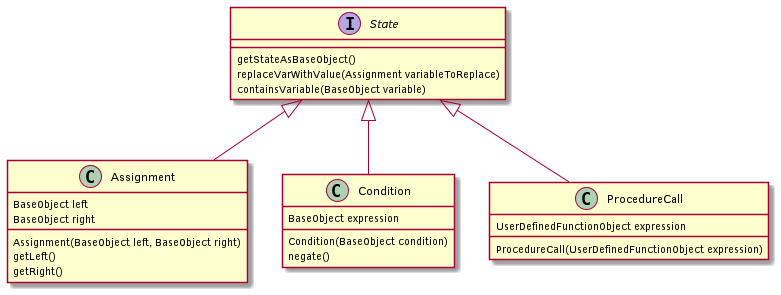
\includegraphics[width=0.85\textwidth]{State}
	\caption{Each \emph{Instruction} in any program may be either represented as an \emph{Assignment}, \emph{Condition} or \emph{ProcedureCall} which encapsulated the expression described in \ref{fig:smtobject}. \emph{Instructions} may be processed into a \emph{BaseObject} during evaluation. \emph{Conditions} and \emph{Procedure} simply contain the expression, whereas \emph{Assignments} translate the left - and right hand side into a \emph{FunctionObject} using \emph{=}.}
	\label{fig:state}
\end{figure}

% AST-Object representation of instructions
Every Instruction will also be represented in an \emph{Abstract-Syntax-Tree}-like notation. Each Symbol, for example a variable, name of a function or any given literal (like numbers and strings), are represented as an \emph{BaseObject}. Functions are, in fact, just a special form of this \emph{BaseObject}, which may contain variables. Functions are not only direct function-/procedure Calls, but also operations (like \emph{+} and \emph{-}). User-defined Functions will also be represented as a special form of the described \emph{FunctionObject} before, which contain the declaration of parameters (since Named Parameters are a language feature of IEC and therefore must be handled correctly), which will be - again - represented as \emph{BaseObjects}. 


\begin{figure}[h!]
	\centering
	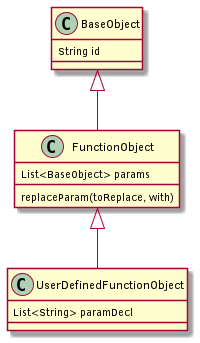
\includegraphics[width=0.2\textwidth]{SMTObject}
	\caption{\emph{AST}-like representation of instructions. This kind of representation makes it easy to work with, since it is a very easy, tree-like data-structure which may be traversed easily. Not only replacing variables and values may be done effortlessly, but also the generation of \emph{SMT-Lib} Code, since this representation is similar to \emph{LISP}.}
	\label{fig:smtobject}
\end{figure}
\section{Analysis}
\label{sec:analysis}
After translation of all \emph{Functions} and \emph{Instructions} the analysis begins. As mentioned in the introduction \ref{cha:finding unreachable code using a smt-solver} of this chapter the \emph{Control-flow Graph} of every function (and procedure) will be traversed. The analysis begins at the single \emph{Begin-Block} of the graph and ends, when all feasible paths reached the \emph{Exit-Block}. \emph{Instruction-Blocks} will be evaluated in Order - the same as a program would execute them. 
For each \emph{Instruction-Block} the \emph{Instructions} will be evaluated. The resulting state must be carried along the analysis and merged correctly to assure valid results. At the end of an \emph{Instruction-Block} a \emph{SMT-Solver} is used to determine if the current state is feasible or not. Infeasible State may be reached by a combination of \emph{Conditions}. If the current state is infeasible, the \emph{next} block must be unreachable, since the \emph{Condition} at the end of an \emph{Instruction-Block} determines which branch the flow follows. 
For the determination, if the current state is feasible or not, the \emph{SMT-Solver Z3}\cite{demouraZ3EfficientSMT2008} was used. The state will be simply translated into the universal, standardized, LISP-like \emph{SMT-Lib} language which most of the common \emph{SMT-Solvers} are able to interpret. 
If an \emph{Instruction-Block} is reachable (at least on one occasion) it will be marked as reachable. At the end of the analysis all remaining \emph{Instruction-Blocks} are marked unreachable.
% TODO: add example for translation
\begin{figure}[h!]
	\begin{GenericCode}
		$i$ $\leftarrow$ 1;
		$x$ $\leftarrow$ 5;
		if ($i$ < $x$) {
			// ...
		}
	\end{GenericCode}
	\begin{GenericCode}
		;; Check if condition evaluates TRUE
		(declare-fun x () Real)
		(declare-fun i () Real)
		(assert (and (= i 1) (= x 5) (< i x)))
		(check-sat)
		; => SAT
	\end{GenericCode}
	\begin{GenericCode}
		;; Check if condition evaluates FALSE	
		(declare-fun x () Real)
		(declare-fun i () Real)
		(assert (and (= i 1) (= x 5) (not (< i x))))
		(check-sat)
		; => UNSAT
	\end{GenericCode}
	\caption{Translation of the IEC-Code. As shown above, each variable must be declared beforehand (therefore the implementation must be aware of the type). The assertion includes the complete state (including \emph{Assignments} and \emph{Conditions}). Conditions are the only part which could lead to an unfeasible result. Every Instruction-Block must contain at least one edge out of the block (with the exception of the \emph{Exit-Block}), but may also contain a second edge, indicating the path if a condition evaluates false. Therefore the condition must be negated.}
	\label{code:translation}
\end{figure}

\begin{figure}[!h]
	\begin{GenericCode}
		$x$ $\leftarrow$ 1;
		$x$ $\leftarrow$ $x$ + 1;
		$i$ $\leftarrow$ $x$;
	\end{GenericCode}
	\centering
	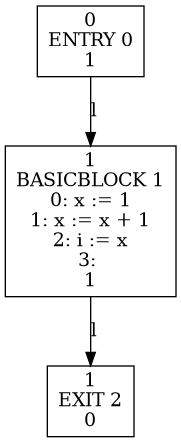
\includegraphics[width=0.2\textwidth]{assignmentsOnly}
	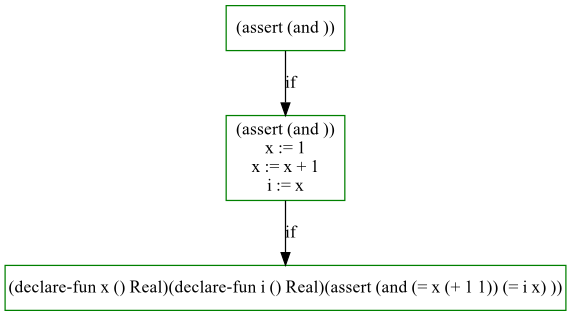
\includegraphics[width=0.5\textwidth]{assignmentsOnly_analysis}
	\caption{TODO: enhance Image on right side. Demonstration of simple Assignments and Reassignments. The resulting \emph{SMT-Lib} Code is displayed on the next Block.}
	\label{fig:assignmentOnly}
\end{figure}

\begin{figure}[!h]
	\begin{GenericCode}
		if ($x$ = 2) 
			y $\leftarrow$ true;
		else
			y $\leftarrow$ false;
	\end{GenericCode}
	\centering
	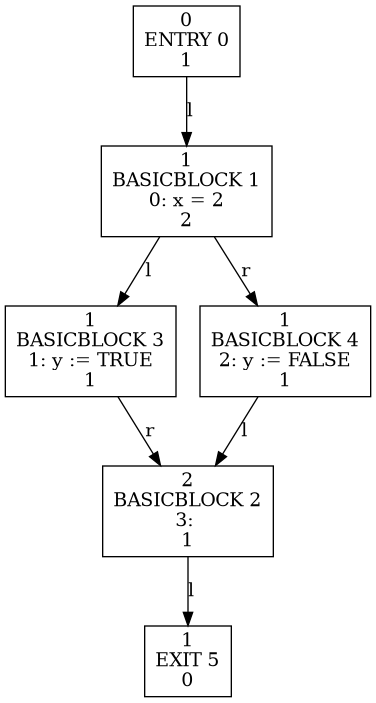
\includegraphics[width=0.2\textwidth]{simpleIf}
	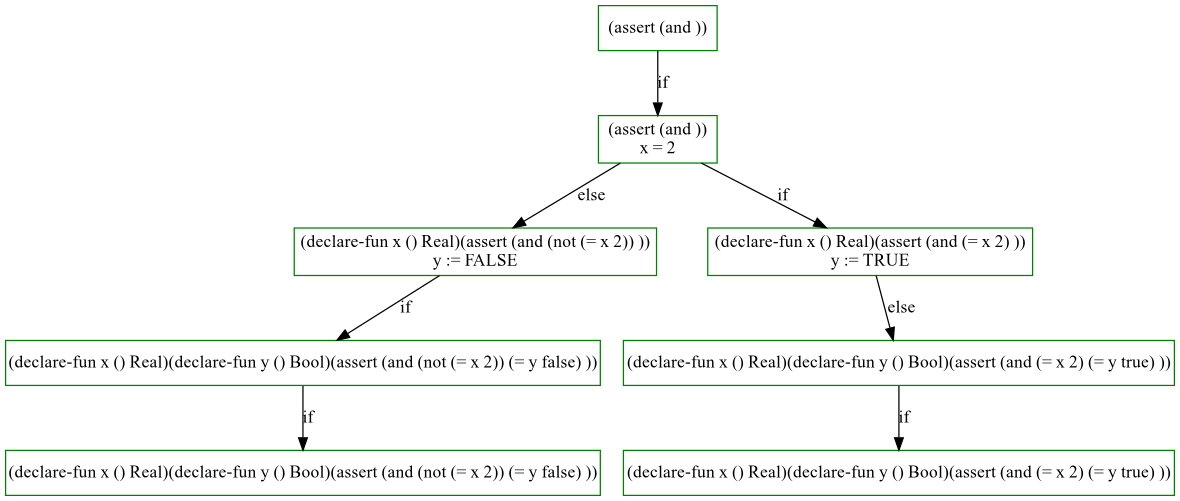
\includegraphics[width=0.5\textwidth]{simpleIf_analysis}
	  \caption{TODO: enhance Image on right side. Simple selection (IF). The flow is divided into to branches - the condition could either be TRUE or FALSE. Each path will be evaluated separately. }
	\label{fig:simpleIf}	
\end{figure}

\begin{figure}[!h]
	\begin{GenericCode}
		for ($i$ $\leftarrow$ 0..$x$) {
			$y$ $\leftarrow$ $i$ + $x$;
		}		
	\end{GenericCode}
	\centering
	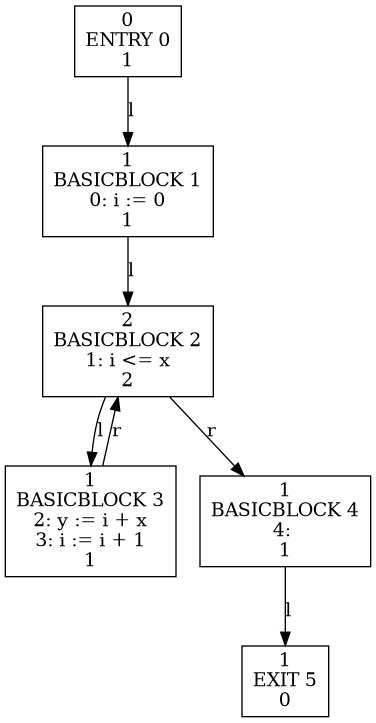
\includegraphics[width=0.2\textwidth]{simpleLoop}
	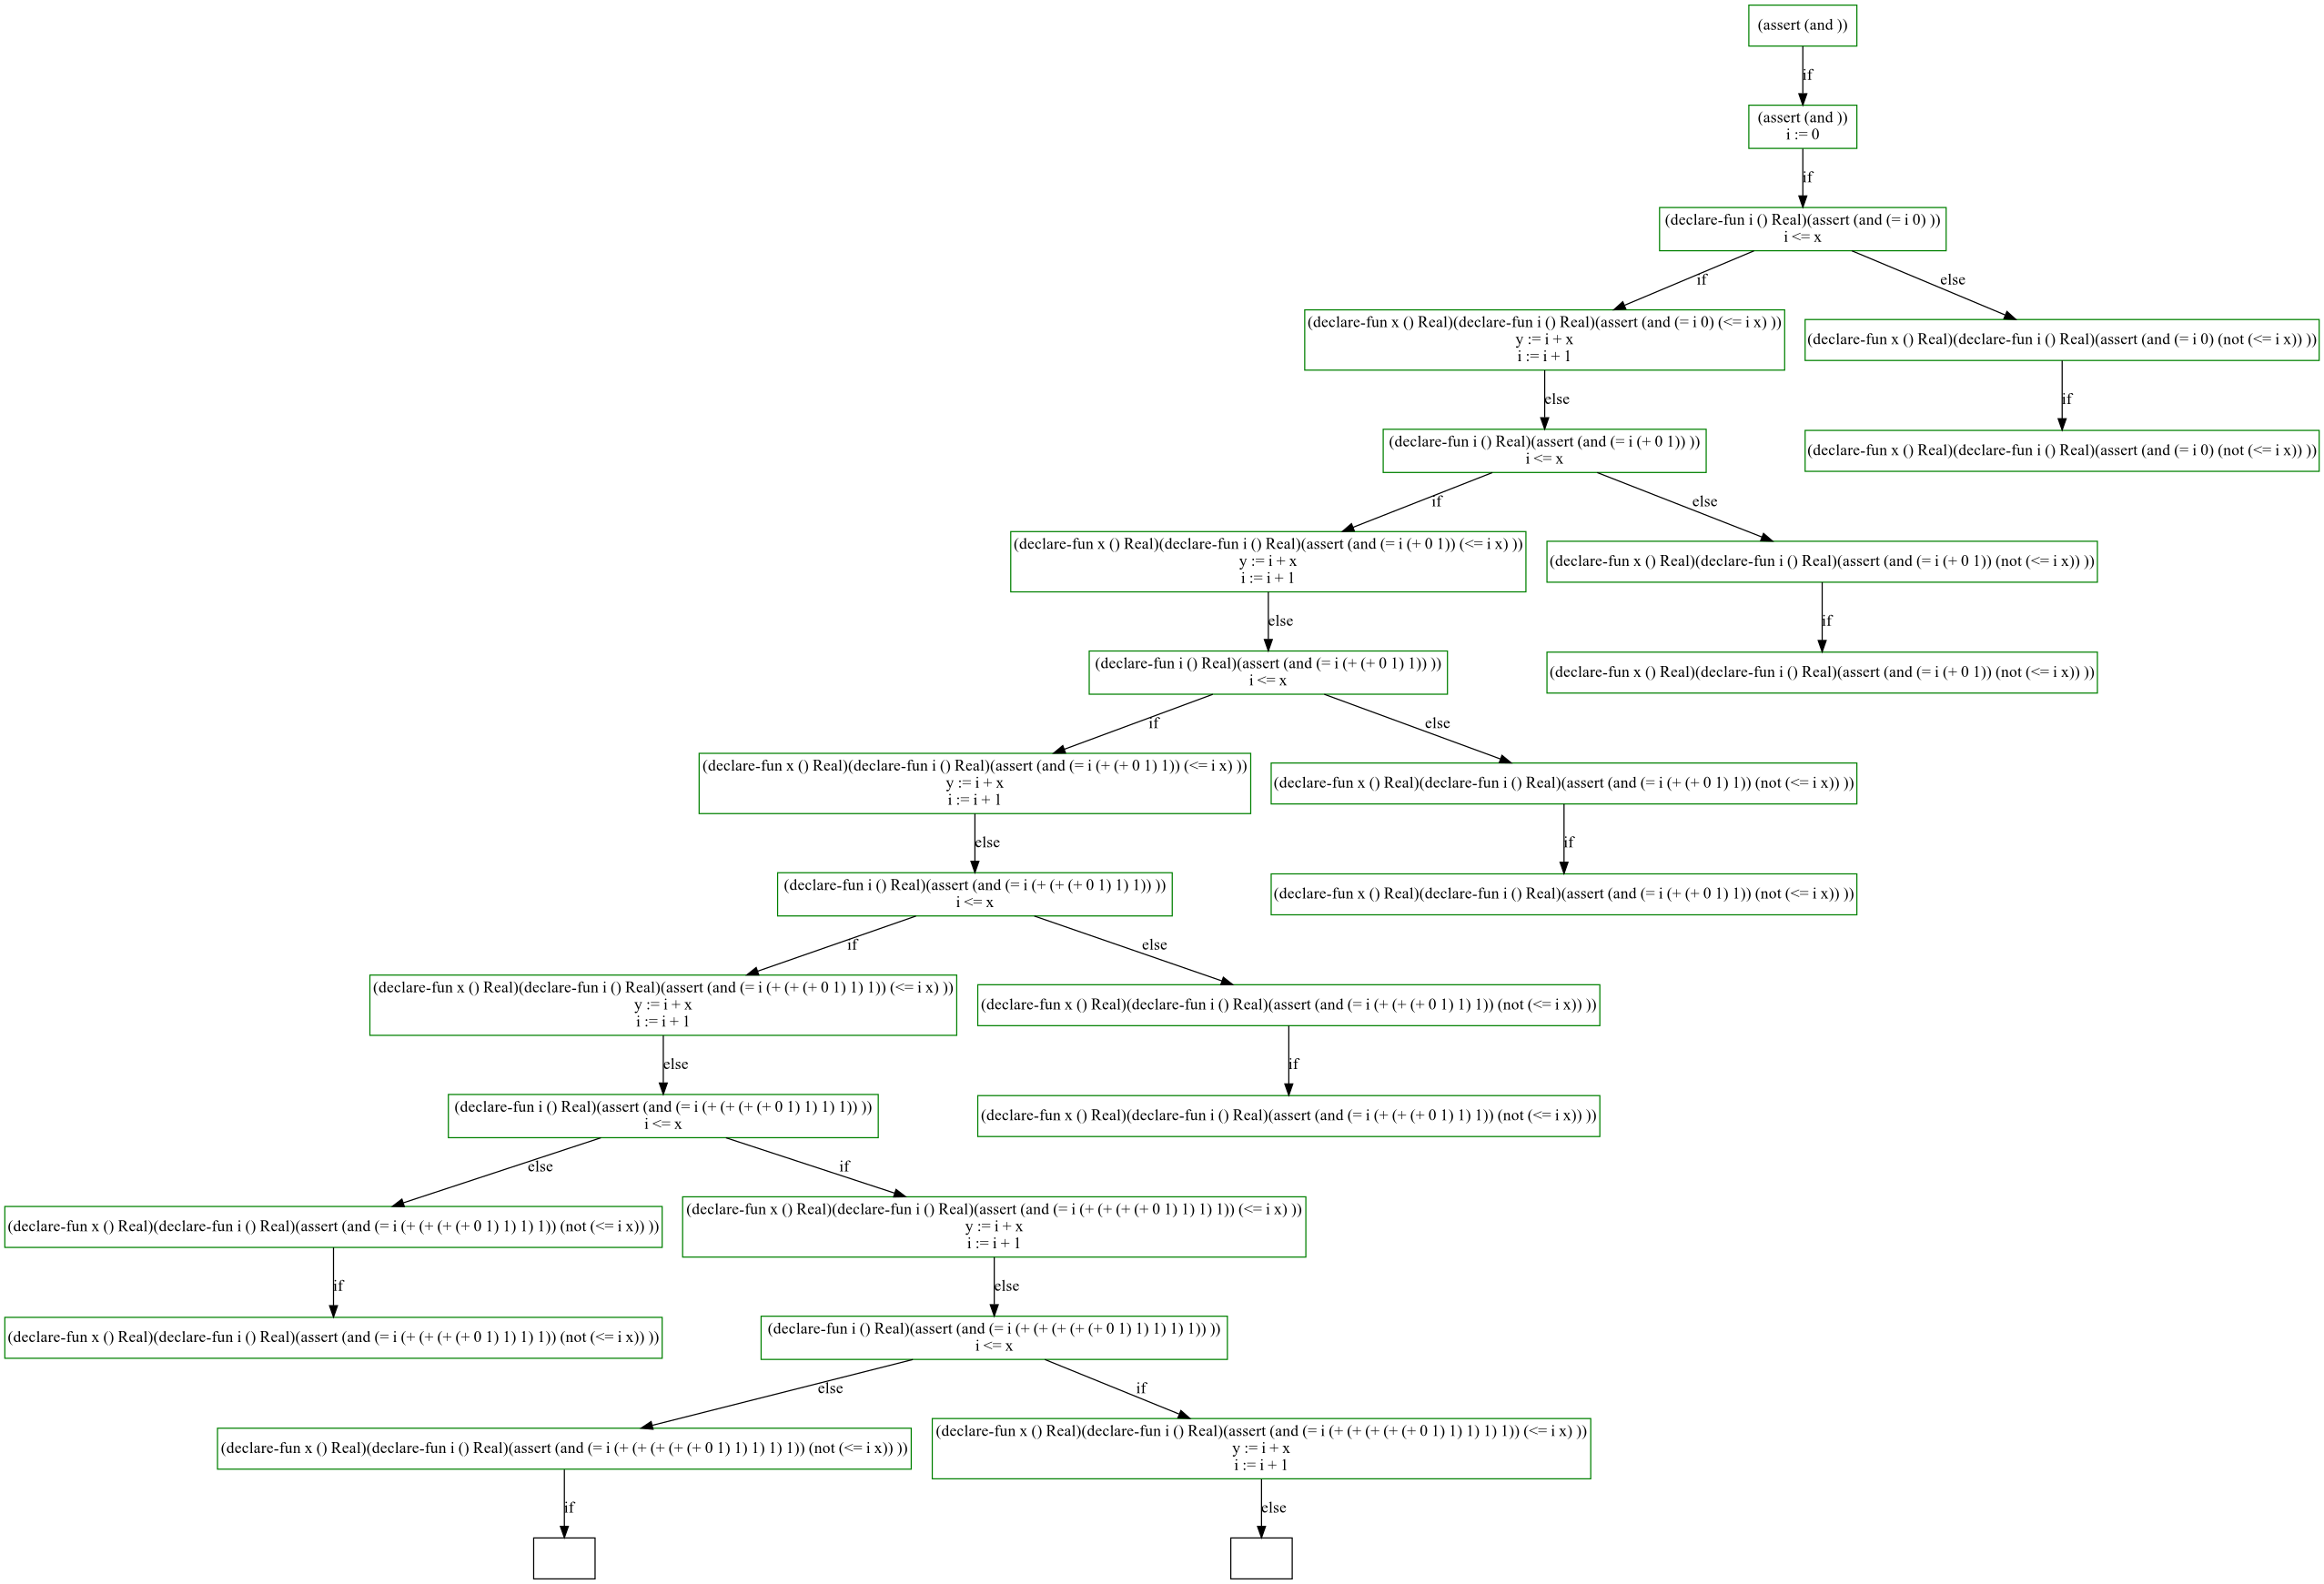
\includegraphics[width=0.7\textwidth]{simpleLoop_analysis}
	  \caption{TODO: enhance Image on right side. After each iteration the condition will be evaluated with the new state again. Every Node is reachable, even tough the analysis stopped prematurely, since the analysis could eventually be indefinitely. }
	\label{fig:simpleLoop}
\end{figure}

\begin{figure}[!h]
	\begin{GenericCode}
		$i$ $\leftarrow$ 1;
		while ($i$ < 10) {
			$i$ $\leftarrow$ 2;
			break;
			$i$ $\leftarrow$ 3;
		}
	\end{GenericCode}
	\centering
	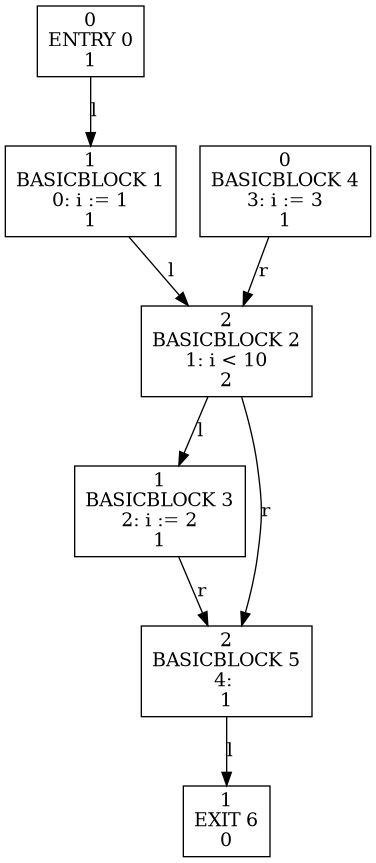
\includegraphics[width=0.2\textwidth]{unconditionalJump}
	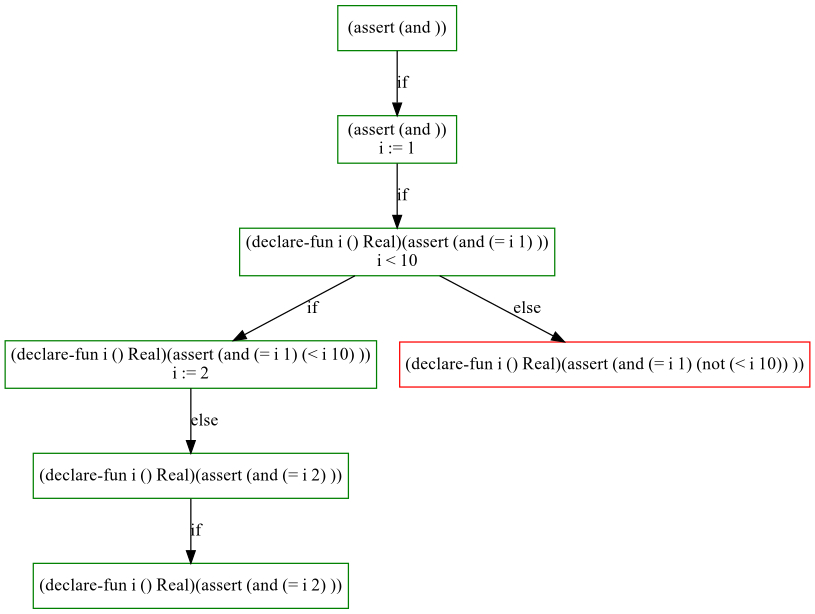
\includegraphics[width=0.5\textwidth]{unconditionalJump_analysis}
	  \caption{TODO: enhance Image on right side. \emph{Instruction-Block} 4 is not reachable, since the flow was interrupted by an unconditional jump.}
	\label{fig:unconditionalJump}
\end{figure}

\subsection{Interpretation of Instructions}
\label{sub:Interpretation of Instructions}
% Handling of and state management
One of the central parts during analysis is the handling of state. Each Instruction must have the same effect as it was executed after compilation. 
As described before, State comes in three forms: Assignment, Condition, Procedure-/Function-call, which all must be handled accordingly. 

\begin{itemize}
	\item Conditions are just added to the state as they are. 
	\item Assignments have to be handled differently. Assignments change the current value of a variable and therefore the path condition is not valid afterwards. It must be reset therefore. 
		If there is any variable on the left side, it must be replaced by its value. Especially cases which contain the same variable on the left and right side must use the values instead of the identifier, since a SMT-Solver does not contain any mechanism for reassignment, but rather a bidirectional Unification. The statement (= x (+ x 1)) will always result in an unsatisfiable state.
	\item Procedure-/Function-calls will be handled as described in \ref{sub:handling procedure and function calls}. If any OUT parameter or the return value will represented as Assignments. 
\end{itemize}

After all Instructions are interpreted, it will be translated into \emph{SMT-Lib Code}, which tests if the next block or blocks are available. 
The state will be passed on until unreachable code is detected or the exit block is reached.

\subsection{Early stopping}
\label{sub:early stopping}
Ideally the analysis takes as much time as possible. Realistically this is not possible to accomplish, therefore mechanisms to stop the computation early must be implemented.
Due to possible mutable state it is not easy to determine values without interpreting the flow of the program. This is the main reason the approach \ref{cha:state of the art} does not detect possible unreachable Code in loops \ref{code:ssa-defect}. 
But being able to find this kind of defects comes with greater execution time. Without proper guards the analysis would take an infinite amount of resources and never find a solution.
\begin{itemize}
	\item One of the simplest mechanisms could be, that as soon as every \emph{Instruction-Block} is marked as reachable, the analysis should stop.
	\item As soon as loops are involved a multitude of different strategies would come to mind. 
	\begin{itemize}
		\item Following the flow of a loop a maximum set amount of time. Note that this approach could lead to false-positives, since the Loop only partly finished. 
		\item Stopping the analysis as soon as too many iterations were made. No false positives will be reported, but the analysis is incomplete.
		\item Resetting the state of every assigned variable inside the body of the loop. Therefore no false positives will be reported, but may overlook some instances of unreachable code.
	\end{itemize}
\end{itemize}

\subsection{Handling Procedure - and Function-calls}
\label{sub:handling procedure and function calls}
Procedure - and Function-calls are handled \emph{Intraprocedural} - meaning return-values are not calculated. That simply means, that every Function-Call just checks, if the declaration contains any (mutable) In- and Out-parameters or is used on the right-hand side of an Assignment.
Either way said variables must reset their state, since the value may change. 
This approach is definitely lighter on the resources, but may not able to detect certain defects which may or may not be obvious to a human. Consider the usage of the identity function. Since the \emph{Intraprocedural approach} does not consider the body of the called function, the state must reset the assigned variable, even tough it does not change.

\subsection{Problems and Barriers}
\label{sub:problems and barriers}
Especially evaluating loops is not gentle on resources and processing power. The number of blocks to evaluate grows exponentially. Naturally loops are very common. In theory this approach could find every instance of unreachable code, only limited by available resources. Multiple strategies \ref{sub:early stopping}  may be applied to reduce the number of iterations.
The consequences of these strategies are, that not every instance of unreachable code can be detected, making this method not necessarily superior to the traditionally implemented approach \ref{cha:state of the art}. 
It may be possible to use some sort of preprocessing and potentially make it possible to evaluate loops only once, which could drastically reduce the execution time and power.
The implementation of such a form of preprocssing must take mutations into account and ideally guarantee the same accuracy.
Without any preprocessing \emph{Interproecural} analysis of \emph{Function-/Procedure-calls} may also increase execution time significantly, since the must be interpreted as well. Here also some sort of preprocessing would be interessting. For example the combination of all influences on return values could be returned. 
Recursive Functions (directly and indirectly) would also lead to an increase of execution time.
